\section{Materia Oscura}\label{sec:materia-oscura}
\subsection{Evoluzione della densità}\label{sec:evoluazione-densita}
Mettendo insieme l'equazione~\ref{eq:friedman} di Friedman, l'equazione~\ref{eq:second-friedman} di accelerazione e l'equazione~\ref{eq:equazione-stato} di stato, mantenendo l'assunzione che $w$ sia costante nel tempo, si ottiene che:
\[
    \rho = \rho_0 {(1+z)}^{3(1+w)} = \rho_0 {R(t)}^{-3(1+w)}
\]
Si osserva che la densità dell'universo sta diminuendo all'aumentare del tempo, al fine di studiare meglio questo andamento scomponiamola nella componente di materia e la componente di radiazione. La prima, che tiene, per l'appunto, conto della materia barionica e della cold dark matter (CDO) ed è di tipo non relativistica ($P<<\rho c^1$), assumendo $w = 0 \Rightarrow P=0$, sarà
\[
    \rho_m = \rho_{m,0}{(1+z)}^3
\]
La seconda, invece, tiene conto della radiazione, la quale avrà una dinamica relativistica, con $w = 1/3$ e di conseguenza
\[
    \rho_{rad} = \rho_{rad, 0}{(1+z)}^4
\]
Si osserva quindi che entrambe le densità fossero estremamente elevate in passato, ma con il tempo sono decresciute con andamenti differenti, in particolare la densità di materia decresce più velocemente di quella di radiazione. Per questo motivo ggi, la densità di materia è circa $1000$ volte maggiore della densità di radiazione $(\rho_{m,0} \sim \rho_{rad, 0}$).

Un'altra componente dell'universo si pensa essere l'energia oscura, ovvero una forma di energia ancora sconosciuta, ma che avrebbe come effetto l'accelerazione dell'espansione dello spazio tempo ($\ddot{R}(t)>0$). Un caso particolare sarebbe quello dell'energia del vuoto, la quale possiede un legame molto stretto con la costante cosmologica ed è caratterizzata da un'equazione di stato con $w = -1$. In particolare se l'energia oscura fosse l'energia del vuoto, allora questa sarebbe ben descritta da un valore $\rho_{\Lambda}$ costante durante tutta l'evoluzione dell'universo. Inoltre, mentre la costante cosmologica venne introdotta da Einstein per imporre un universo statico, poi annullata da Hubble per spiegare l'evoluzione dell'universo, ora la presenza di questa energia oscura impone di tenere conto di una costante cosmologica che impone un'accelerazione in questa espansione.

Gli effetti di un'espansione in accelerazione può essere visto considerando un universo dominato da materia, assumendo quindi che
\[
    \rho_{m} = \rho_{m, 0}{(1+z)}^3 = \rho_{m,0}{R(t)}^{-3}
\]
riscrivendo l'equazione di Friedman come segue.
\[
    {\dot{R}(t)}^2 = - kc^2 + \frac{8\pi G \rho_{m,0}}{3R(t)} + \frac{\Lambda {R(t)}^2}{3}
\]
La cui derivata diventa:
\[
    {\ddot{R}(t)}^2 = -\frac{4\pi G \rho{m,0}}{3{R(t)}^2}+ \frac{\Lambda {R(t)}^2}{3}
\]
dove si osserva che il termine di auto-gravitazione concorre con un contributo negativo all'accelerazione dell'espansione, mentre quello contenente la costante gravitazionale ad un aumento. Se quindi questi due termini si bilanciano, si avrebbe un espansione dell'universo costante.

Conoscendo la dipendenza temporale della densità di ogni componente del fluido cosmico, dalla determinazione del valore della densità al tempo presente, è possibile costruire l'andamento totale partendo dall'origine dell'universo. Distinguiamo, in particolare, cinque componenti fondamentali: di radiazione ($\rho_{rad, 0}$), di materia barionica ($\rho_{b, 0}$), di materia oscura ($\rho_{DM, 0}$) e di energia oscura ($\rho_{\Lambda, 0}$, le quali concorrono all'andamento totale quella totale ($\rho_{0}$).

\subsection{Cosmic Microwave background (CMB)}\label{sec:CMB}
Il \textit{Cosmic Microwave background} ci permette di studiare l'universo nei suoi primissimi istanti di vita, in figura~\ref{fig:CMB1}, ad esempio, mostra la distribuzione di temperatura. Si osserva che questa non è perfettamente uniforme, ma sono presenti delle minuscole fluttuazioni di circa $\SI{100}{\micro K}$ in una scala angolare di $\sim 1\si{\degree}$, il cui scarto relativo è $\Delta T/T \sim 10^{-5}$.
\begin{figure}
    \centering
    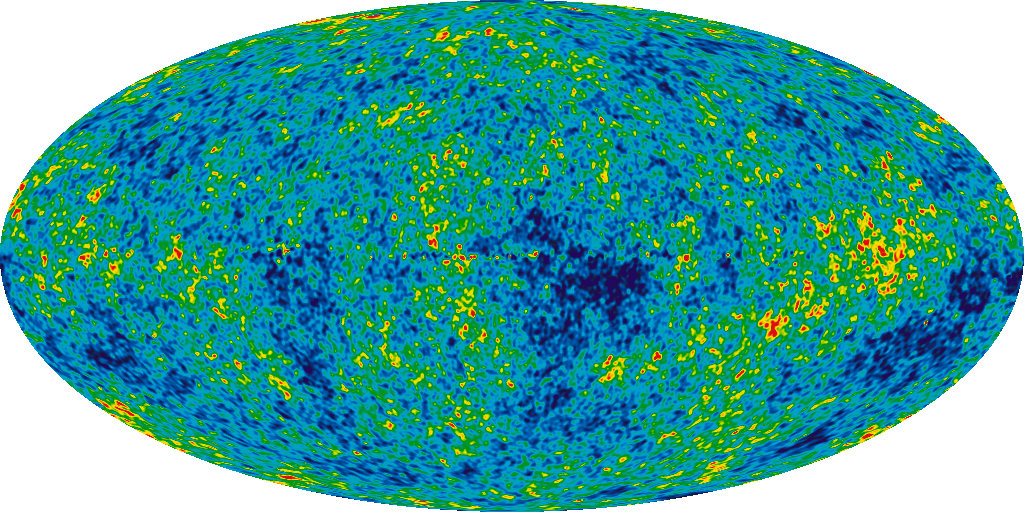
\includegraphics[width = 0.6\textwidth]{immagini/CMB1.png}
    \caption{L'immagine mostra il Cosmic Microwave background su tutto l'arco celeste.}\label{fig:CMB1}
\end{figure}

La misura della temperatura permette di stabilire la densità di radiazione che permea una determinata sezione di universo. Infatti, Se
\[
    \rho_{rad} = \frac{4\sigma T^4}{c^3}
\]
con $\rho_{rad}$ la densità di massa della radiazione, $T$ la temperatura e $\sigma = \SI{5.67e-8}{W.m^{-2}.K^{-4}}$ la costante di Stefan-Boltzmann, allora la stima della temperatura della CMB al giorno d'oggi è $T=\SI{2.725}{K}$, che equivale a una densità $\rho_{rad, 0} \simeq \SI{4.9e-34}{g.cm^{-3}}$. Questa appare decisamente più piccola rispetto alla densità critica $\rho_{c,0}$, definita nella sezione~\ref{sec:equazione-friedman}, per cui $\Omega_{rad,0} \approx 5\times 10^-5 \sim 0$. La dimensione delle fluttuazioni relative di temperatura implicano inoltre una geometria dello spazio piatta, poiché dallo CMB si osserva in media una radiazione uniforme e altrimenti si avrebbero fluttuazioni che prendono una sezione angolare maggiore. Questo vuol dire che $\Omega_0 = 1 \Rightarrow \rho_0 = \rho_{c,0}$ con un accuratezza di circa il $2\%$.

Attraverso l'analisi di Fourier dello spettro di potenza del cosmic microwave background permette di calcolare l'esatta densità di materia barionica contenuta nell'universo, ottenendo che $\Omega_{b,0} = 0.049$, come mostrato in figura~\ref{fig:baryon}.
\begin{figure}
    \centering
    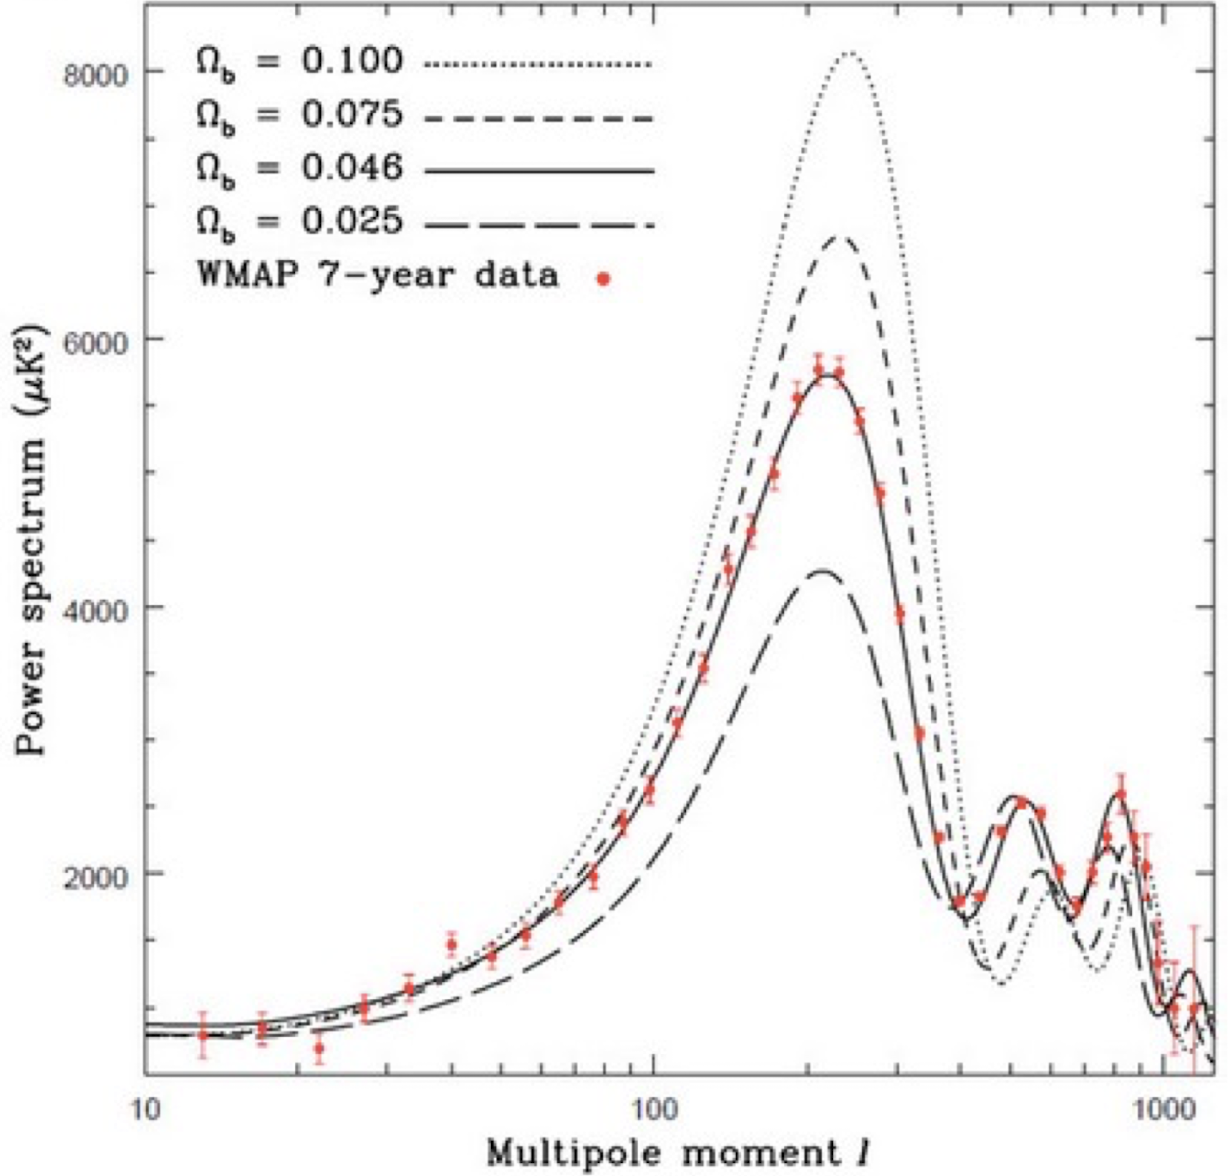
\includegraphics[width=0.4\textwidth]{immagini/barioni.png}
    \caption{La figura mostra le varie distribuzioni per l'intensità dello spettro del CMB in funzione della lunghezza d'onda angolare (in gradi) per vari valori di densità barionica, osservando che il modello migliore è proprio quello per $\Omega{b,0} = 0.049$.}\label{fig:baryon}
\end{figure}

Dall'osservazione del gravitational lensing delle galassie, inoltre, si è misurata la densità di materia oscura presente nell'universo, ottenendo un valore pari a $\Omega_{DM,0} = 0.26$. Per della materia che compone l'universo si ha che la DM ne rappresenta l'$84\%$. Sommando tutti i contributi, però, si ottiene che
\[
    \Omega = \Omega_{rad,0} + \Omega_{b,0} + \Omega_{DM,0} = 0.31
\]
manca per ciò una frazione di densità di massa pari a $0.69$ per arrivare a $\Omega_0 = 1$. Tale contributo è stato assunto provenire da quella che viene chiamata \textit{Energia Oscura}, che permea l'intero universo. La prova diretta di questo fatto valse il Premio Nobel del 2011 a Perlmutter, Schmidt e Riess. Attraverso lo studio di supernove a distanza variabile, ottennero che il miglior modello prevedeva valori per le densità di massa pari a $\Omega_M = 0.3$ e $\Omega_\Lambda = 0.7$, usando quello che viene detto \textit{Diagramma di Hubble}, ovvero un piano distanza-redshift (figura~\ref{fig:diagramma-hubble}).
\begin{figure}
    \centering
    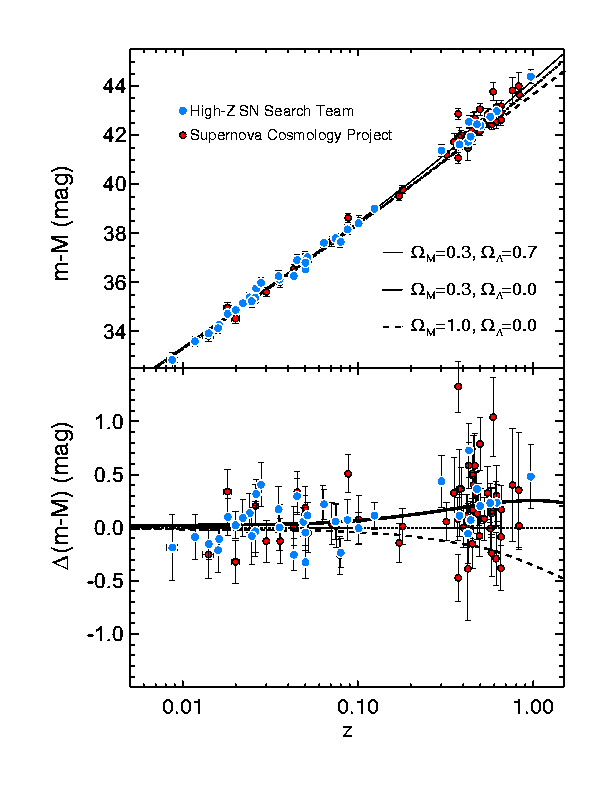
\includegraphics[width=0.4\textwidth]{immagini/hubble_diagram.png}
    \caption{Lo studio è stato eseguito prendendo supernove di tipo I.a, poiché anche a grandi redshift (distanze), permettono di poterle osservare e misurare la loro magnitudine apparente, risalendo alla distanza conoscendo quella assoluta. Questo perché, come visto nel paragrafo~\ref{sec:supernove}, tutte le supernove hanno luminosità uguale.}\label{fig:diagramma-hubble}
\end{figure}

Per cui la materia ordinaria, che abbiamo imparato a conoscere e che continua a celare molti misteri, non è che il $5\%$ del contenuto dell'universo. 